\chapter{Dude Where's My Psyker?}

\begin{wrapfigure}{O}{\figwidth}
	\begin{center}
		
\includegraphics[width=\figwidth]{pics/3/5.png}
	\end{center}
\end{wrapfigure}
This is the ongoing tale of a bunch of guardsmen who got drafted into the Inquisition after their regiment was reduced to a mere 37 men by a combination of Orks, Heretics, more Orks, Tyranids, and of course, their own leadership. 
Currently, they’re working for an Inquisitor that is the 40k equivalent of Professor Oak; he provides teams and missions to Interrogators who need to get some leadership experience before becoming full Inquisitors. 
The lot of these guardsmen is rather thankless, they’re matched up with five other less combat focused team members, assigned to an Interrogator, and sent out to fight the enemies of the Imperium.

Our story starts with Nubby and Twitch vainly trying to open up the locked exit to the shuttle after being told that their new squad contained three psykers in addition to an assassin, tech-priest, and the Interrogator himself. 
Sarge is screaming internally as he remembers that the last psykers he worked with accidentally summoned a blood storm and turned into a daemonhost the second they tried to do anything. 
Doc is captivated by the sight of a fat little man-child chewing on a seat’s headrest. 
Heavy has decided that this is all above his paygrade and is making himself comfortable by lying across a row of seats. 
The Interrogator explains that the team is on its way to find out why a planet has not been supplying psykers to the Black Ships. 
One of the psykers asks Sarge to stop screaming, it’s making it hard to think.
>Current Psychic Phenomena Count: 0
>Current Perils of the Warp Count: 0 \todo{fix}

\begin{wrapfigure}{O}{\figwidth}
	\begin{center}
		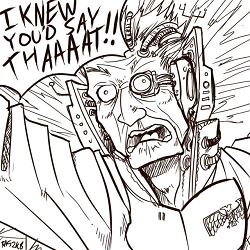
\includegraphics[width=\figwidth]{pics/3/6.png}
	\end{center}
\end{wrapfigure}
So no shit there we were, stuck on a small ship with three psykers, on our way to perform a top to bottom search of an entire planet, all for the sole purpose of finding MORE psykers. 
We did not have high hopes for this mission. Hell, some of us had serious concerns about whether we’d even still be sane when we got there.

The journey itself wasn’t so bad. Instead of being guests on a navy vessel our Interrogator actually had his own small ship. 
Sure, almost all the space was taken up by our Interrogator's huge ass cogitator array, but at least we didn’t have any navy ratings trying to take our weapons away, or bitching at us for setting trip-wire traps in the corridors. 
The problem was the people we had to make the journey with.

We didn’t like any of the psykers. 
One was a smarmy tool, who spent far too much time talking and making himself look pretty; then there was the weasley creep, who constantly scanned everyone’s thoughts and ratted to the boss; and finally, there was this psychotic man-child who would occasionally throw telekinetic temper-tantrums. 
We called them Face, Snitch, and Nutjob respectively. 
Compared to these guys, the snooty social assassin chick and the incredibly antisocial tech-priest weren’t that bad. 
The Interrogator was infinitely worse. 

Our Interrogator was adept-path and apparently some sort of data wizard. 
It took an entire ship just to carry all of his cogitators and he loved those machines like they were his children; unfortunately the bastard wasn’t a complete shut-in. 
Instead of staying in the dark with his cogitators, he constantly held meetings and forced us all to attend. 
Not a day would go by without him calling us together to update everyone on what little clues he’d found, or check up on how we were preparing for the mission, or lecture us on proper inquisitorial behavior. 
It was horrible.

\begin{wrapfigure}{O}{\figwidth}
	\begin{center}
		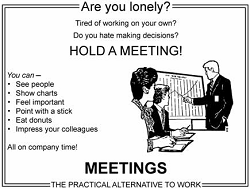
\includegraphics[width=\figwidth]{pics/3/7.png}
	\end{center}
\end{wrapfigure}
On our previous mission we happily ignored everyone else on our team while they happily did likewise. 
This time, we had an Interrogator who had never used a gun in anger giving us unwanted advice about combat drill, kit loadout, regulatory compliance, and freaking etiquette. 
This was all done in a tone of smug benevolence; he understood that we were just dim-witted manual laborers and couldn’t be blamed for not being as smart as he was, that’s why it was his duty to do all the hard thinking for us. 
The cherry on top of this was Snitch, who would report what we were THINKING to the boss. 
Every time those lectures filled us with murderous rage the little weasel would go and tell on us, then we’d get a second lecture on proper attitude towards authority. God Emperor we hated him.

Eventually we arrived at the planet which had earned the Inquisition’s attention by providing the Black Ships with nothing but pathetically weak psykers completely unsuited for any use whatsoever. 
There were probably dogs out there with more psychic talent than the strongest psyker sent to the ships, but when the Black Ships had scanned the planet there were no unsanctioned psykers running around, so they took the pathetic tithe and left. 
Now we were here to find out where all the psykers that should have been on a planet of this size had gone. 
The gist of all the little briefings we suffered through was that a disappearance on this scale meant that we were either dealing with corruption in the government, a massive cult, some kind of psyker-eating daemon, or Eldar. 
This meant that unless proven otherwise, we had to assume that EVERYONE was in on it, so until the Interrogator got some sort of evidence we wouldn’t have any outside support.

\begin{wrapfigure}{O}{\figwidth}
	\begin{center}
		
\includegraphics[width=\figwidth]{pics/3/8.png}
	\end{center}
\end{wrapfigure}
The posh assassin chick and Face did all the social legwork. 
They would circumspectly shake people down for information while we loomed in the background, or preferably down the street at a cheap diner. 
Apparently they were very good at it, since everyone aside from us thought they were absolutely delightful to be around. 
At the end of each day they would transcribe everything they found and beam it up for the Interrogator to process. 

The other information gathering team involved the tech-priest and Snitch hanging around in the equivalent of an unmarked van. 
They spent all day driving around hacking wireless networks, scanning peoples thoughts, and dumping all the information back to the boss in orbit. 
We got to drive the van and fetch snacks.

We didn’t all get to leave the ship, one or two of us were always stuck at base since it was apparently our job to babysit the Nutjob psyker. 
It really was babysitting too, ‘cause we’d have to clean up the messes he made, get food for him, calm him down when he threw a fit, and entertain him when he got bored and started pulling rivets out of the walls with his brain. 
Poor Doc got that job more than anyone else, he just wasn’t very good at saying no. 
Aside from that though, it was an improvement over the trip out there. 
We were occasionally able to get away from our teammates and whoever was backing up the social team got to visit some pretty high-class parties. 
It was always a nice opportunity to snag some good food and, in Nubby’s case, pocket the silverware.


\begin{wrapfigure}{O}{\figwidth}
	\begin{center}
		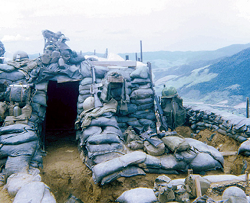
\includegraphics[width=\figwidth]{pics/3/9.png}
	\end{center}
\end{wrapfigure}
After a while, the Interrogator called us together and informed us of his brilliant deductions and masterful analyses. 
These involved money trails, newfound political power, falsified ship manifests, and other stuff we didn’t really care about. 
It all boiled down to, “Someone in the government is selling the psykers off planet”. % TYPO changed punctuation
Once our Interrogator was done explaining his genius, he had everyone but himself rebase to a few floors of apartments, located in one of the larger cities on the planet. 
After the team was settled in, he sent us out to take some long, hard looks at a bunch of the nearby banks. 

We enjoyed being away from him and his constant meetings, and quickly turned the building into a proper guard barracks. 
Which is to say that Twitch wired the place up with dozens of traps, Nubby started fencing stolen goods out of the garage, and the rest of us built a set of barricades between us and the outside world, as well as between us and the rest of our damned team. 
It felt good to be home.

\begin{wrapfigure}{O}{\figwidth}
	\begin{center}
		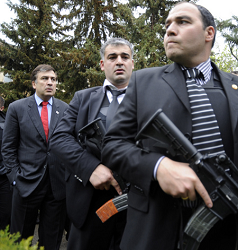
\includegraphics[width=\figwidth]{pics/3/10.png}
	\end{center}
\end{wrapfigure}
Before long, word came down that the Interrogator had identified the operation’s banker and the whole ground team was sent off to get some answers out of him. 
So while Heavy hung out in the van with the socially unacceptable members of the team and ignored the ugly little man prodding his brain and demanding candy, the rest of us infiltrated the bank. 
That is to say we put on suits, which succeeded in making us look exactly like guardsmen in suits, and marched behind Face and the assassin into one of the planet’s largest banks. 

There was a little bit of trouble getting through security, which was entirely our fault. 
All of us had kept our las-rifles underneath our suits, and Twitch was still carrying a few det packs. 
We weren’t very good at disguises. 
Luckily, between Face doing some psyker stuff and the tech-priest’s hackvan messing with the security systems, we got in fine. 

After we were past security, Face and the assassin greased a few palms and screwed with a few minds. 
Before long, we all sat down to a nice discussion and tea-time with the banker. Well, they sat, us guardsmen stood around and looked ominous. 
Various falsified credentials were shown, psychic tricks were used, and a discrete uplink was attached to a cogitator, then everyone left happy and healthy. 
We decided to exit via the back way so as not to trouble security again, and also because Nubby had wheeled out the tea-trolley when we left.

\begin{wrapfigure}{O}{\figwidth}
	\begin{center}
		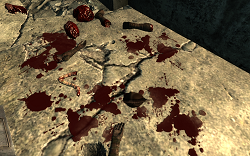
\includegraphics[width=\figwidth]{pics/3/11.png}
	\end{center}
\end{wrapfigure}
The boss and the rest were pretty excited about what was found on the banker’s cogitator. 
The next few days were spent in relative peace while the Interrogator worked with the rest of the team to map out a web of corruption and bribery. 
This lasted right up until Snitch called us one evening and said a large group of hitmen was moving through the empty floor below us.

We were locked and loaded within seconds and started laying fire into the hitmen from multiple sides before they even hit the edge of the perimeter. 
We had good cover, good firing lines, knowledge of local terrain, superior weaponry, much better training, and the element of surprise. 
It was a slaughter. 
The last three of them were pinned down by Heavy and Twitch while the rest of us flanked them when everything went dark, and horrific screaming started. 
When the lights returned all the hitmen, dead or alive, had been reduced to chunky salsa and we could all hear Nutcase giggling upstairs.

This killed the mood, everyone eyed the psyker nervously as we packed up our shit and got the hell out of there before the authorities showed up. 
We elected to exit via the garages in a cargo truck while the rest of the team used the shuttle on the roof. 
None of us wanted to be anywhere near the Psykers after that show, also Nubby and Twitch didn’t want to leave anything behind.
>Psychic Phenomena Count: 1
>Perils of the Warp Count: 0\todo{fix}

\begin{wrapfigure}{O}{\figwidth}
	\begin{center}
		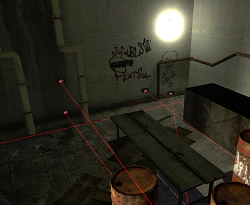
\includegraphics[width=\figwidth]{pics/3/12.png}
	\end{center}
\end{wrapfigure}
We rebased to another almost identical set of apartments and went about guardifying it again, except this time Twitch was given free reign on the entire buffer floor instead of just the entrances and windows. 
While this meant that entering our base via the main entrance took about fifteen minutes and carried a very real risk of grisly death, we knew that people were actively trying to kill us.
Also, we didn’t want to depend on anyone who turned bodies into chunky salsa and giggled about it for our perimeter security. 
The rest of the team started using air transport exclusively after the assassin nearly lost a hand when she didn’t follow Twitch’s entry instructions correctly.

After a few days at our new base doing scan trips and otherwise laying low, Snitch found a young nascent psyker powerful enough to be worthwhile.
So our team of elite inquisitorial agents started staking out a toddler. 
Our unmarked vans followed the kid day and night, from his hab, to the daycare, to the playground, and everywhere else you might take a toddler. 

Imagine five heavily armed men all clustered around a screen watching a kid being pushed on a swing while behind them an undeniably creepy bugger relays what everyone in the playground is currently thinking and a psychotic man-child picks his nose and mutters to himself. 
Eventually our weird stakeout paid off: a bunch of suits showed up and grabbed the kid and his mother.

\begin{wrapfigure}{O}{\figwidth}
	\begin{center}
		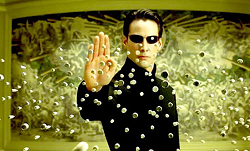
\includegraphics[width=\figwidth]{pics/3/13.png}
	\end{center}
\end{wrapfigure}
So no shit there we were, five guardsmen and two psykers in the middle of a playground chasing a bunch of g-men carrying a struggling woman and a small child.
The woman and child were screaming, the g-men were calling for backup, our psykers were yelling about one of the g-men being a blunter, and while we all had our guns out none of us wanted to open fire in the middle of a playground. 
We were gaining on them (being a sprinter is a survival trait in any guardsman), but right as we reached them one of them slapped a button on their chest and another one of them started to float into the air as the surrounding area was covered with frost. 
We all immediately slammed into an invisible wall and were scattered across the ground, while Snitch stopped and started muttering himself and gesturing.

None of us wanted to be in the middle of a psyker fight, so we flanked the invisible shield, left Heavy to cover the enemy Psyker, and resumed the chase. 
The g-men had gone to ground in a playscape and opened fire on us with small arms, but were having trouble because the child was apparently emitting random bursts of static electricity. 
We decided that survival was more important than civilian casualties and returned fire from whatever cover we could find, and since we were damned good at our jobs thing went pretty poorly for the g-men. 
We nailed most of them in the first few volleys which convinced the last few to keep their heads down while we flanked them. 
Behind us Heavy was laying stubber fire into the enemy psyker’s shield and Snitch was pressing him hard, then with a little pop the enemy psyker disappeared.

\begin{wrapfigure}{O}{\figwidth}
\begin{center}
	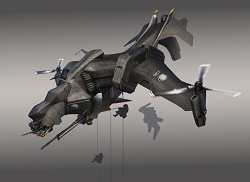
\includegraphics[width=\figwidth]{pics/3/14.png}
\end{center}
\end{wrapfigure}
While Heavy and Snitch watched the spot where the Psyker had been we rushed the remaining g-men. 
Our Interrogator was helpfully reminding us over the vox that he wanted prisoners, so we charged in to beat the shit out of the last few survivors. 
Unfortunately at this point their backup arrived in the form of an unmarked government flier, which immediately began to lay down some serious suppressive fire. 
This was higher stakes than we were ready for, so we bugged the hell out while the remaining g-men piled in with the kid and his mother. 
The flier wasn’t done with us though: as soon as its doors were closed, it lifted off and got ready to do a strafing run.

We hit the dirt and dodged the first pass like true guardsmen, while behind us the enemy psyker had reappeared with another pop and the fight resumed.
This time the fight was over in seconds, the Nutjob had finally caught his fat ass up with us and with a little ~schlorp~ the enemy psyker turned inside-out.
That done with, both the psykers and Heavy turned their attention to the flier, which decided that it was time to cut its losses and got the hell out of there. 
As we got back up out of cover the Interrogator called us to tell us that the assassin and Face had successfully tagged the flier with a tracer and the tech-priest would shortly be picking us up to assault whatever facility it landed at.

>Psychic Phenomena Count: 3
>Perils of the Warp Count: 1\todo{fix}

\begin{wrapfigure}{O}{\figwidth}
\begin{center}
	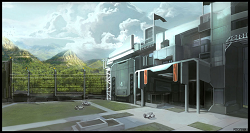
\includegraphics[width=\figwidth]{pics/3/15.png}
\end{center}
\end{wrapfigure}
Apparently some minor detail about the g-men or the flier finally gave the Interrogator the evidence he needed to safely call in official support. 
After he was done bitching at us for not capturing anyone, or stopping the flier, or whatever else we did wrong, our Interrogator told us a squad or two of Arbites would be assisting us. 
Nubby was understandably nervous about being around what were nominally law enforcement officers, and none of us were happy when the Interrogator explained that he was only bringing in the Arbites because he thought we were incompetent, but overall this news was well received by us guardsmen. 
More bodies between us and incoming fire is always welcome, doubly so if they had heavy armor and good fire discipline.

The facility we landed at was large, grim, and obviously a shuttleport; therefore our job in this raid was to capture any available information about where the shuttles would be going. 
So while two squads of Arbites had fun clearing the place room by room with judicious use of shotguns and shockmauls, we kept a secure perimeter around the rest of our team as they uplinked cogitators and mind-scanned people. 
Aside from a few runners and idiots too dumb to surrender, we didn’t have any excitement until one of the Arbite squads found the psyker holding area.

As the Arbites closed in, one of the g-men apparently decided that the situation was unsalvageable and released the psykers. 
Under the cover of a dozen psychically gifted children freaking the hell out, they punched through the Arbite squad and headed right towards us, or more likely the flier we were examining. 
We opened fire as the heavily armed g-men entered the hangar and had them pinned in the hallway until Sarge and Heavy’s cover got blown apart by a fireball. 
Once again we found ourselves caught in a psyker duel; it was three on three, and this time, Nutjob wasn’t curbstomping them.


\begin{wrapfigure}{O}{\figwidth}
\begin{center}
	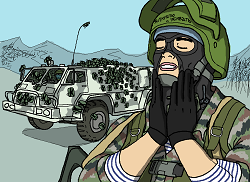
\includegraphics[width=\figwidth]{pics/3/16.png}
\end{center}
\end{wrapfigure}
The fight seemed evenly matched, our psykers stood there and grimaced a lot and occasionally manifested horrible smells or small earthquakes, their psykers sat in cover and did likewise. 
We didn’t have line of sight on any of them and when we tried to toss in a grenade, it got slapped back at us halfway through its arc. 
We weren’t exactly sure what to do, but after the fourth creepy occurrence we decided it was time to use our initiative to end this shit before someone summoned a daemon.

Sarge appropriated a nearby forklift, drove it outside the hangar, and then we slapped a bunch of det packs on it. 
We turned it toward the outside wall of the hallway the psykers were holed up in, put a brick on the pedal, and blew the entire hallway into rubble before anyone noticed what was going on. 

It surprised the hell out of us when the dust cleared and two of the psykers were still there, hiding under a shield, but it didn’t last long after that. 
With a hellish bang, one of the psykers shot into the air and splattered against the shield and the last psyker immediately turned inside out. 
We could hear the Nutjob giggling back in the hangar.

>Psychic Phenomena Count: 8
>Perils of the Warp Count: 2\todo{fix}


\begin{wrapfigure}{O}{\figwidth}
\begin{center}
	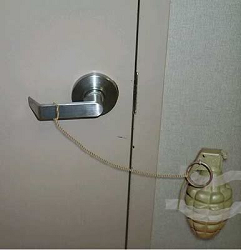
\includegraphics[width=\figwidth]{pics/3/17.png}
\end{center}
\end{wrapfigure}
That was the last of the resistance. 
We poked through the military hardware that was left behind while the rest of our team did inquisitorial stuff to the surviving g-men and their cogitators. 
After they were finished, we packed up our loot and headed back to base to rest and re-arm while the Interrogator played with all the data we got for him. 
We were assured that before long he’d know where the psykers had been sent from the processing facility, and were told to get ready to launch another assault as soon as he had a target. 

Being guardsmen we knew that the best way to prepare for an assault is to eat a good meal and catch as much sleep as possible, so as soon as our kits were prepped we all hit the sack while the rest of the team watched the perimeter. 
This meant that we were all deep asleep, with the exception of Twitch who merely dozed with with his las-gun pointed at the door and the safety off, when a second assassination team got through our outer perimeter.

The enemy must have seen the remains of their last team and decided that the psykers were the primary threat, because this team had at least one untouchable with it. 
Unfortunately for them, untouchables don’t do anything to stop booby traps. 

The whole team had slowly cleared a small path across the floor that Twitch had trapped and reached the big expensive security door that led to our makeshift barracks.
They formed up behind their best infiltrator and got ready to storm the place as soon as he hacked the door controls. 
Then the door opened, and they had exactly .25 seconds to express surprise that anyone would tape several short-fuse grenades to the inside of a top-of-the-line security door.


\begin{wrapfigure}{O}{\figwidth}
\begin{center}
	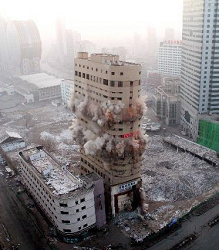
\includegraphics[width=\figwidth]{pics/3/18.png}
\end{center}
\end{wrapfigure}
This woke us all up and, Twitch being Twitch, he’d put an entire clip and two frags into the open doorway before anyone else was upright. 
He probably didn’t hit anyone since the six grenades taped to the inside of the security door had vaporized everyone near it, but he sure as hell convinced their rearguard to start falling back. 
Not that it did them any good: before the rest of us were on our feet Twitch hit the remote detonator for the every single mine he’d placed below us. 
The entire buffer floor was blown to shrapnel, taking the rest of the assassination team with it and setting off alarms up and down the entire block. 
Luckily, the building was non-flammable and sturdily built, so aside from a very rude awakening no one we really cared about was hurt.

Sarge decided that nap-time was over, so we kitted up and waited for the word from our Interrogator. 
Before long it came, he’d pinpointed a Rogue Trader that was receiving the psykers and carrying them to off-world slave markets. 
A joint naval and Arbite force would meet us in orbit, and we would board the trader before they made their escape. 
Our primary objective was to capture the senior crewmembers and find their contact within the local government. 
Secondary objectives included: retrieving any psykers currently on the ship, capturing the navigational and financial logs, and “Not blowing the ship up like you blew up our base; are all guardsmen this incompetent?”

\begin{wrapfigure}{O}{\figwidth}
\begin{center}
	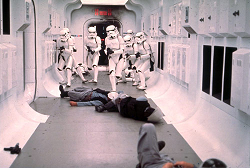
\includegraphics[width=\figwidth]{pics/3/19.png}
\end{center}
\end{wrapfigure}
So no shit there we were, on a naval boarding shuttle, on our way to capture a Rogue Trader and his retinue from a ship filled with captive psykers. 
We were not exactly enthusiastic about our odds of survival. 
Rogue Traders have a reputation for being, or at least employing, very scary people. 
Plus, an entire ship of untrained ones was a terrifying thought, ours were bad enough alone. 
Still, we were guardsmen, facing certain death for unappreciative superiors is what being a guardsman is all about.

None of us really enjoyed the shuttle trip, the pilot was clearly terrified and the evasive maneuvers made us all nauseous. 
We half expected to be blown out of space before we got to the ship, but we landed on the hull without incident and cut our way into the interior. 
While we did this, several other navy and Arbite shuttles were doing likewise. 
This was not a subtle attack, so it was hardly surprising that before we got ten feet in the ship’s alarms started to go off.
We knew our business though, and mowed down all opposition before they got a shot off on us. 

The assault was going well for all of the teams. 
We’d seized the engines and main batteries, the main hangars were on the verge of surrender, and the tech-priest was pretty sure he’d located the bridge. 
Seizing the initiative he remotely hacked all the entrances to lock open so they couldn’t be shut against us.
Unfortunately those turned out to actually be the doors to the psykers’ isolation cells, the second he opened them everything went to hell. 
Literally.

\begin{wrapfigure}{O}{\figwidth}
\begin{center}
	
\includegraphics[width=\figwidth]{pics/3/20.png}
\end{center}
\end{wrapfigure}
Ghostly images filled the air, the frescos on the walls started weeping blood, unearthly screaming came from every direction, and a stench that put even Nubby’s lack of hygiene to shame emanated from the air vents. 
Our psykers moved forward to try and sort things out before the entire ship got sucked into the warp or something, but we wanted nothing to do with a section of spaceship filled with supernatural darkness and constantly fluctuating gravity. 
We still had a mission though, and since the psychic activity was blocking vox communication Sarge took operational command.

We needed to get to the bridge, which the rather embarrassed tech-priest assured us was definitely just a little farther past the psyker holding area. 
Once there we needed to find the Rogue Trader, subdue him, and hit him until he ratted on his buddies. 
The problem was that even though there were other passages to the bridge that didn’t go through the psyker cells, the psychic spillover had turned that entire section of ship into a No Man’s Land. 
Just walking in there would be suicide, but Sarge figured that there was a safe way to cross the hellscape if we only could find the right people. 

Sarge was pretty sure that any ship carrying a bunch of unhappy psykers would have at least one untouchable on board, just in case something like this happened.
All we needed to do was find out where they were, and convince them to take a walk with us.

So we had our tech-priest do a quick scan to find out if any areas nearby weren’t experiencing paranormal activity, then went to go knock on some doors. 
Sure enough, we found two untouchables hanging out in a cabin speculating on what all the fuss was about. 
One of them tried to make a fight of it and got shot for his trouble, but the other understood that in times like this, all men need to come together and serve the Emperor. 
So we cocooned him in duct tape, threw him over Heavy’s shoulder, and set off for the bridge.

\begin{wrapfigure}{O}{\figwidth}
\begin{center}
	
\includegraphics[width=\figwidth]{pics/3/21.png}
\end{center}
\end{wrapfigure}
The walk was really quite pleasant as long as you ignored the dents, stains, puddles, and complete absence of any living creature. 
We waltzed right up to the bridge without any opposition, and found it locked down tighter than a Sororitas Convent when the guard was in town on leave. 
While the locked doors might have posed a problem for some of the other boarding groups, Nubby had helpfully attained several of the cutting tools that the shuttle crew had used to open up the outer hull. 

So with the tech-priest’s help we found a section of wall which was much thinner than the blast door and started cutting our way in. 
Sadly, even with a breaching charge to help with the final step, a lascutter is not quick or subtle. 
All we found in the bridge after we flashbanged the shit out of it and stormed in was a bunch of empty seats and a locked door labeled “Escape Pods”

We used the ship’s vox to contact the Boss and explain the situation. 
After he was done bitching at us, especially the poor tech-priest, he decided that given our lack of success he would track the Trader’s escape pod instead of just blowing it out of the sky. 
We were to go get our damned psykers back and get ready to raid wherever the Trader finally went to ground.

So with our duct taped untouchable in tow, we went back into the psychic no man’s land and started sorting shit out. 
The DTU really trivialized everything, it was just a matter of walking up to the psykers, having Doc tranq them, then tossing them on the pallet Heavy was pushing. 
Occasionally we’d run into a minor daemon, or crazed crew member, or obvious daemonhost, but between the DTU and a liberal dose of las-fire nothing posed a real threat. 
We eventually collected all the surviving psykers (a few of them were inside out, freaking Nutjob) and found our three psykers a little worse for wear, but ready to go after the Rogue Trader as soon as we knew where he was going.

>Psychic Phenomena Count: 23
>Perils of the Warp Count: 5\todo{fix}

\begin{wrapfigure}{O}{\figwidth}
\begin{center}
	
\includegraphics[width=\figwidth]{pics/3/22.png}
\end{center}
\end{wrapfigure}
The pallet full of sedated psykers was turned over to the Arbites along with the DTU. 
We were sad to see him go, he was like a big sticky teddybear that kept us all safe and happy, but he had to stay with psykers so we handed him over to the Arbites and headed for the shuttle. 
The Interrogator voxed us with directions to pick up the assassin, who had spent the whole mission getting her nails done or something, and report to an Arbite precinct near some big government mansion. 
Our Interrogator had used his INCREDIBLE skills and BRILLIANT mind to track the Rogue Trader here, and oh so cleverly pinned Secretary Such and Such as the mastermind of this whole mess. 
Our job was to quietly go in and capture the Secretary and the Rogue trader so they could be used by the Inquisition to sort all this out without causing a massive scandal or minor war.

So while the Arbites put up a very discrete perimeter and the tech-priest worked with some local enginseers to quietly shut down the mansion’s communications, the rest of our team planned our infiltration. 
By this point Sarge was done with everyone’s shit and vetoed several complex ruses suggested by the assassin and Face. 
Eventually they just gave up and the team was disguised as a group of heavily armed guardsmen and some dangerously unstable psykers.

\begin{wrapfigure}{O}{\figwidth}
\begin{center}
	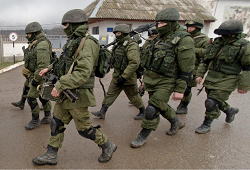
\includegraphics[width=\figwidth]{pics/3/23.png}
\end{center}
\end{wrapfigure}
These weren’t exactly the best disguises, but we felt pretty sure that everyone could act their part. 
Grumbling about obstinate guardsmen and stupid plans, the rest of the team dressed themselves up as officers and good ol’ fashioned sanctioned psykers. 
For our part we tacked on the insignia of a local regiment and caught some sleep while the rest got their costumes in order. 

When everyone was dressed up we walked right through the mansion’s security pretending to be a local general dropping off some extra protection for his good friend the Secretary. 
The poor sod was out of his mind with panic, he was calling in every favor he had to fortify his mansion and we fit right in with all the others. Our credentials weren’t even checked, as soon as we claimed to be reinforcements we were waved past security and let inside. 
He even invited the ‘General’ up to his office to personally thank him for his generosity. 

We walked right into the Secretary’s office and presented ourselves to him while the Rogue Trader stood behind him and stared at us boggle eyed. 
Nothing good can last forever though, and after a few seconds of speechlessness the Rogue Trader called the Secretary a bloody idiot and opened fire.

\begin{wrapfigure}{O}{\figwidth}
\begin{center}
	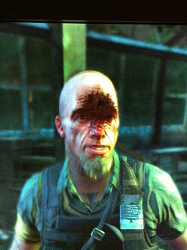
\includegraphics[width=\figwidth]{pics/3/24.png}
\end{center}
\end{wrapfigure}
The Rogue Trader was a little late though, by the time he drew his weapon the assassin had grabbed the Secretary and we had already killed several bodyguards. 
We signalled the Arbites to move in, grabbed some cover, and started a two way firefight between the Trader and security reinforcements. 
We had him well pinned and had started to flank him when the far door burst open and the Trader’s retinue entered the fight, two of them were already glowing. 
Once again we found ourselves stuck in the middle of a damned psyker duel. 
Meanwhile, the Arbites moved in to detain everyone, and without direct orders from the Secretary none of the security forces felt inclined to argue with the Arbite’s APCs. 

Back inside, Heavy was mowing down reinforcements with his stubber, Twitch was nailing anyone who left cover, and the rest of us were steadily advancing on the Trader and his psykers. 
Surprisingly, the two enemy psykers were holding off all three of ours, and aside from a few phenomena neither side appeared to actually be doing anything. 
Eventually our slow advance got us a good shot on the Trader and his retinue, pushing the psykers to try something desperate.

Face collapsed, but one of the Trader’s psykers burst into flame, taking a pair of retainers with him. 
In response, Nutjob and Snitch doubled down on the last psyker, until suddenly Nutjob fell to the ground screaming and one of the last retainers did likewise.

Suddenly the retainer got to his feet and tackled the last enemy psyker to the ground and started beating the shit out of him while giggling. 
While we all watched this, Nutjob got to his feet, drew his sidearm and shot Heavy in the back of the head.

\begin{wrapfigure}{O}{\figwidth}
\begin{center}
	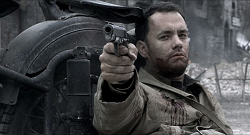
\includegraphics[width=\figwidth]{pics/3/25.png}
\end{center}
\end{wrapfigure}
A second shot was fired at Twitch, but a quick dodge saved him. 
Unfortunately, the second he stopped covering the Trader, a round hit him in the back. 
While this happened, Sarge and Nubby downed the last retainer and the Trader disappeared with a loud crack.
Immediately afterward, the enemy psyker stopped moving, Doc ran towards Twitch and Heavy, and both the possessed retainer and Nutjob collapsed again. 

While Doc started patching up Twitch, Snitch collapsed in exhaustion, and Nubby headshot the psyker and the retainer that had been attacking him. 
Sarge scanned the room for the Trader, and with a tired giggle Nutjob began to sit up.
Immediately the injured Twitch drew his sidearm and emptied an entire clip into the little bastard. 
No one commented on this.

\begin{wrapfigure}{O}{\figwidth}
\begin{center}
	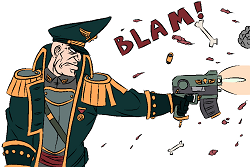
\includegraphics[width=\figwidth]{pics/3/26.png}
\end{center}
\end{wrapfigure}
Sarge and Nubby slowly approached the door to the bathroom attached to the office. 
Right as they reached it a voice from inside announced “I would like to surrender to the Inquisition, and put myself and my ship at their disposal in this current investigation.” 
Both Sarge and Nubby ignored this and started prepping a breaching charge. Before they finished, they heard the assassin, who had been hiding with the Secretary behind a filing cabinet, comm the Interrogator and tell him that the target had been captured and the Trader was surrendering. 
The Interrogator ordered Sarge to “Accept the gentleman’s surrender and escort him to the shuttle.” 
With a weary sigh, Sarge removed the charge and relayed the message. 

After a few seconds the Rogue Trader opened the door and smugly declared, “I knew we could work together, this was such a tragic misunderstanding-” whereupon Nubby yelled “Ee’s got a gun!” and Sarge blew his head off. 

The Interrogator was not happy.

\begin{wrapfigure}{O}{\figwidth}
\begin{center}
	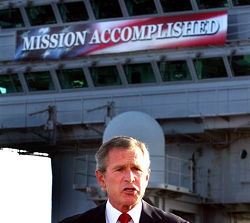
\includegraphics[width=\figwidth]{pics/3/27.png}
\end{center}
\end{wrapfigure}
That was the end of our part of the investigation. 
Doc got Twitch stable and patched everyone else up, while Sarge collected Heavy’s body and Nubby looted the corpses.

It was sort of awkward sitting there waiting for the all-clear from the Arbites. 
The Secretary was moaning and crying in a very annoying way, and the rest of the team kept shooting us death glares while they struggled to restrain him.
We offered to help, but they refused us for some reason. 
The mood was not improved by Nubby making some truly horrific noises as he tried to pry something out of the Trader’s corpse. 
In the end he had to borrow Doc’s bonesaw.

Eventually the Arbites finished clearing the mansion and a team escorted us back to their precinct. 
A flier came and picked up the Secretary along with the assassin, Snitch, and Face, and hauled them off to some secure facility somewhere. 
We weren’t told anything, we were definitely on the Interrogator’s shit-list.

>Final Psychic Phenomena Count: 28
>Final Perils of the Warp Count: 7\todo{fix}

\begin{wrapfigure}{O}{\figwidth}
\begin{center}
	
\includegraphics[width=\figwidth]{pics/3/28.png}
\end{center}
\end{wrapfigure}
We hung out with the Arbites for a few hours and they were nice enough to give us some food and help sew Twitch up while we waited. 
After a while shuttle came for us, as well as, to our surprise, the tech-priest. 
It took us to the Interrogator’s ship. 
The ride up was pretty somber: Heavy was dead, both his and Nutjob’s corpses were in the hold, and we knew the Interrogator was furious with us. 
Not even Nubby’s jokes about the selling price of secondhand gold teeth or his reenactment of the Rogue Trader’s death could cheer us up. 

When we got back to the ship we were treated to a long lecture about how our incompetence had ruined the Interrogator’s carefully laid plans. 
We were told how Sarge’s disobedience had removed a vitally useful source of information, how our poor decision making had killed a valuable teammate, and how the tech-priest’s mistake on the ship had jeopardized the entire mission. 
He also made several remarks about our general behavior, attitude, hygiene, and education, then finally pointed out that if only we had acted as professionally as the rest of the team Heavy would still be alive. 
If the bastard didn’t have remote control of the ship’s security servitors, Sarge would have probably killed him.

In the end we were ordered to pack up and return to the shuttle, we would be returning to Oak’s ship on a naval transport while the investigation was finished with the aid of the Arbites and local Ad-Mech. 
A secure data-slate containing a summary of the investigation so far as well as a detailed critique of our performance was sent along with us.
It came with a dire warning that Oak would be expecting the slate and any attempt to accidentally lose it would go poorly. 
So we packed up our gear and Heavy and boarded our shuttle. 
However, as a final afterthought, we propped Nutjob’s corpse upright in the bathroom where it would hopefully scare the shit out of that damned Interrogator.

\begin{wrapfigure}{O}{\figwidth}
\begin{center}
	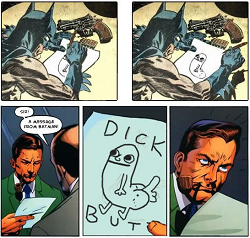
\includegraphics[width=\figwidth]{pics/3/29.png}
\end{center}
\end{wrapfigure}
The trip back was a lot better than the trip out. None of the navy boys bothered us and we bonded with the tech-priest over our mutual hatred of that bastard Interrogator. So aside from Sarge’s usual drills, we mostly just lounged around and came up with ideas for how to change the report after the tech-priest finished hacking the “secure” data-slate.

Very few pieces of technology can resist a tech-priest with a month of travel time on his hands, before the trip was even half done he had it cracked open and ready for a little judicious editing. 
There was a strong sentiment to wipe the whole thing and replace it with a picture of a butt and a note that said “blah blah blah I’m a gigantic tool blah blah blah,” but cooler heads prevailed. 
We simply removed all negative references to ourselves from the report, and rewrote the disciplinary note to simply say that we were no longer needed and were being released back to Oak. 
As an afterthought, we went through the entire report and dialed the Interrogator’s self-praise up to eleven. 
We hoped it would help him come off as a complete tool to anyone who read the report.

\begin{wrapfigure}{O}{\figwidth}
\begin{center}
	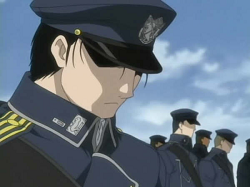
\includegraphics[width=\figwidth]{pics/3/30.png}
\end{center}
\end{wrapfigure}
Eventually we arrived back at Professor Oak’s giant spacefaring inquisitorial school, which was currently orbiting some random agri-world. 
We dropped off the data-slate, got debriefed, and went to go find our fellow guardsmen. 
Sure enough, there were a few of them holding down the little section of the ship that we had claimed back when we arrived. 
We got together, shared some stories, and planned a suitable funeral for Heavy. 
We called up the tech-priest and found our other cogbro still hanging out in engineering, so we invited them both down to the planet with us. 
Then we got Heavy out of storage, “requisitioned” a shuttle, and headed down to the agri-world to give him a proper sendoff.

In the morning the cogbros helpfully hauled all of our hungover asses back onto the shuttle and got us back aboard before anyone noticed we had left. 
That done with, we settled in for a few well deserved weeks of R\&R. 
On some days, a squad would come back with tales of success or failure and occasionally missing a few men. 
Other days, a runner would come down and a squad would head out or a new one would be pieced together. 
Eventually, the squad’s R\&R time ran out, so we packed our bags and waited for the runner to come for us.

\begin{wrapfigure}{O}{\figwidth}
\begin{center}
	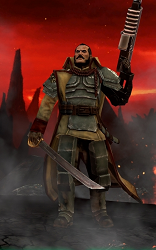
\includegraphics[width=\figwidth]{pics/3/31.png}
\end{center}
\end{wrapfigure}
The runner didn’t come though. 
Instead, one day as we lounged in our makeshift barracks, a tall man ducked into the room. 
He wore dress greens and positively reeked of Officer. 
In a chipper voice he greeted us and invited our squad and “that strapping young fellow with the sword” to join him on a little expedition. 
He said he was going into a combat zone and thought that we’d enjoy a chance to get back into action and solve “a few little military problems that are right up our alley, wot wot!”

So with a weary sigh, we gathered up the one man in the regiment dumb enough to prefer a sword over a good old fashioned las-gun and followed our new Interrogator to the shuttle.











